% Options here are passed to the article class.
% Most common options: 10pt, 11pt, 12pt
\documentclass[10pt]{datasheet}

% Input encoding and typographical rules for English language
\usepackage[utf8]{inputenc}
\usepackage[english]{babel}
\usepackage[english]{isodate}

% tikz is used to draw images in this example, but you can
% also use \includegraphics{}.
\usepackage{graphicx}
\usepackage{float}
\usepackage{subcaption}

% These define global texts that are used in headers and titles.
\title{MX03: Bob The Builder Loop}
\author{Andrews54757}
\tags{everything-bagel, music}
\date{25 December 2024}
\revision{Revision 1}
\begin{document}
\maketitle

\section{Features}

\begin{itemize}
    \item{Repeatedly outputs the Bob The Builder theme song}
\end{itemize}

\section{Applications}

\begin{itemize}
    \item{Inspirational music.}
\end{itemize}

\section{General Description}
The MX03 Bob The Builder Loop generates music to the tune of the \href{https://www.youtube.com/watch?v=HdVg-2jn2OU}{Bob The Builder} theme song.

``Can we fix it? Yes we can!"
\vfill\break

\begin{figure}[H]
    \centering
    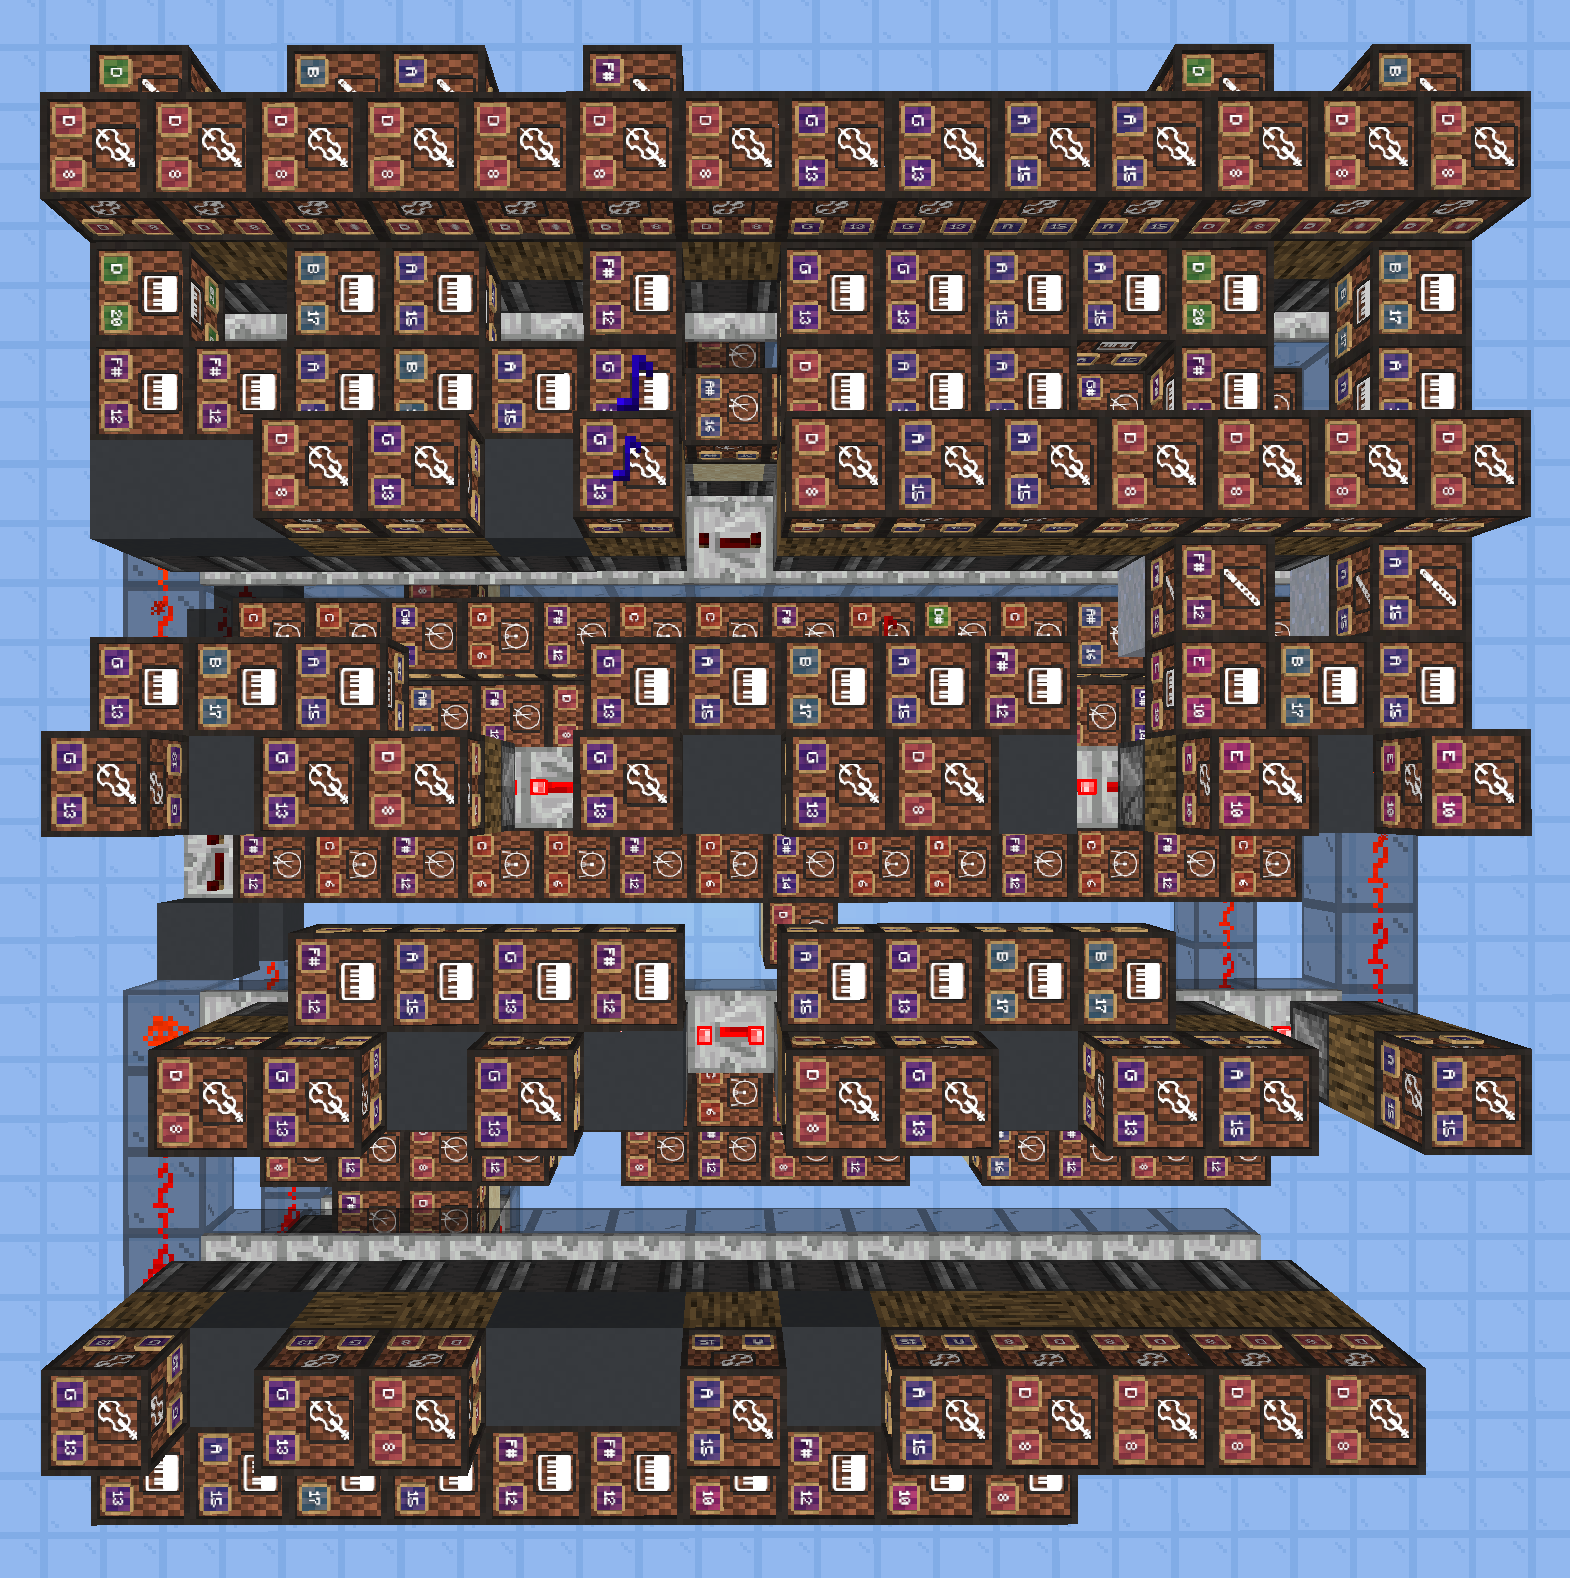
\includegraphics[width=0.48\textwidth]{bob.png}
    \caption{\centering Bob The Builder Loop}
\end{figure}

% For wide tables, a single column layout is better. It can be switched
% page-by-page.
\onecolumn

\section{Device Specifications}

\begin{table}[H]
    \caption{Inputs}
    \begin{tabularx}{\textwidth}{l | c | X}
        \thickhline
        \textbf{Name} & \textbf{Range} & \textbf{Description} \\
        \hline
        Lock & 0-1 & Plays music when power is removed from the lock input. \\
        \thickhline
\end{tabularx}
\end{table}

\begin{table}[H]
    \caption{Outputs}
    \begin{tabularx}{\textwidth}{l | c | X}
        \thickhline
        \textbf{Name} & \textbf{Range} & \textbf{Description} \\
        \hline
        Music & Sound & Outputs the Bob The Builder theme music. \\
        \thickhline
\end{tabularx}
\end{table}

\begin{table}[H]
    \caption{Device Specifications}
    \begin{tabularx}{\textwidth}{l | c c c | c | X}
        \thickhline
        \textbf{Parameter} & \textbf{Min.} & \textbf{Typ.} & \textbf{Max.} &
        \textbf{Unit} & \textbf{Conditions} \\
        \hline
        Music Length & 384 & - & - & gt & Time between loops. \\
        \hline
        MC Version & 1.13 & 1.20.4 & - & MCV & Latest version at time of writing: 1.21.4\\
        \hline
        Dimensions & & 15 x 10 x 16 & & Blocks & \\
        \thickhline
\end{tabularx}
\end{table}

\section{Testing Data}
\begin{table}[H]
\caption{Executed Tests}
\begin{tabularx}{\textwidth}{l | X}
    \thickhline
    \textbf{Test} & \textbf{Result} \\
    \hline
    Music test & Device was able to produce the desired music. \\
    \thickhline
\end{tabularx}
\end{table}

\section{Download Information}
\begin{table}[H]
    \caption{Download Information}
    \begin{tabularx}{\textwidth}{l | l | l | X}
        \thickhline
        \textbf{Identifier} & \textbf{MC} & \textbf{File} & \textbf{Description} \\
        \hline
        MX03 & 1.20.4 & \href{https://github.com/Soontech-Annals/Archive/blob/8413f90a054b6c415703bae02badeba7541344f6/Archive/everything-bagel/MX03\%20Bob\%20The\%20Builder\%20Loop/MX03\_Bob\_The\_Builder\_Loop.litematic?raw=1}{MX03\_Bob\_The\_Builder\_Loop.litematic} & Schematic of device. \\
        \hline
        \thickhline
    \end{tabularx}
\end{table}

\end{document}

